\chapter{KẾT QUẢ THỰC NGHIỆM VÀ THẢO LUẬN}
\label{chuong5}
\label{ch:ket_qua_thuc_nghiem}

\vspace{-1.5cm}

\begin{quotation}
    \noindent
    \small\textit{
    Chương này trình bày kết quả đánh giá AutoShotV2 so với các mô hình cơ sở trên các bộ dữ liệu thực nghiệm, phân tích Precision/Recall/F1, phân rã cho từng thành phần cải tiến, các lỗi điển hình và khả năng tổng quát hóa qua miền dữ liệu. Phần cuối chương trả lời trực tiếp các câu hỏi nghiên cứu đã đặt ra ở Chương~\ref{ch:tong_quan}.
    }
\end{quotation}
\vspace{1em}
\section{Tổng quan các nhóm thực nghiệm}

Trước khi đi vào từng bảng chi tiết, Bảng~\ref{tab:experiment_group_overview} tóm tắt các nhóm thực nghiệm chính được sử dụng trong chương này. Bảng chỉ báo cáo F1-score đại diện để người đọc nắm toàn cảnh; các chỉ số Precision, Recall, TP/FP/FN và phân tích chi tiết được trình bày ở các mục sau. Bảng đầy đủ tất cả thí nghiệm được đặt tại Bảng~\ref{tab:all_experiments_master} trong Phụ lục~\ref{app:per_video_results}.

\begin{table}[H]
\centering
\caption[Tổng quan các nhóm thực nghiệm chính]{Tổng quan các nhóm thực nghiệm chính. Các giá trị là F1-score; mỗi dòng dùng protocol riêng nên chỉ dùng để định hướng, không so sánh trực tiếp ngoài phạm vi ghi chú.}
\label{tab:experiment_group_overview}
\small
\setlength{\tabcolsep}{3pt}
\renewcommand{\arraystretch}{1.15}
\begin{tabular}{L{4.3cm}C{1.8cm}C{1.8cm}C{2.1cm}L{4.0cm}}
\toprule
\textbf{Nhóm thực nghiệm} & \textbf{SHOT} & \textbf{BBC} & \textbf{ClipShots} & \textbf{Ghi chú} \\
\midrule
\ExperimentOverviewRows
\bottomrule
\end{tabular}
\end{table}

\section{Kết quả chính trên SHOT và các bộ dữ liệu bổ sung}

Bảng~\ref{tab:autoshotv2_results} tổng hợp F1-score của AutoShot, TransNetV2 và các biến thể AutoShotV1/AutoShotV2 khi đánh giá trên ba tập dữ liệu SHOT, BBC và ClipShots.

\begin{table}[H]
\centering
\small
\setlength{\tabcolsep}{4pt}
\renewcommand{\arraystretch}{1.2}

\begin{tabular}{L{5.0cm}C{2.2cm}C{2.2cm}C{2.4cm}}
\toprule
\textbf{Phương pháp} & \textbf{SHOT} & \textbf{BBC} & \textbf{ClipShots} \\
\midrule
\MainComparisonRows
\bottomrule
\end{tabular}
\caption[So sánh F1-score các mô hình trên SHOT, BBC và ClipShots]{So sánh F1-score của các mô hình trên SHOT, BBC và ClipShots. Hàng ``AutoShot theo báo cáo'' lấy từ bài báo gốc~\cite{zhu2023autoshot}; các hàng ``tự chạy lại'' là kết quả tái lập trong khóa luận với điểm lưu trọng số công khai và quy trình đánh giá thống nhất. AutoShotV1 là cấu hình trung gian chỉ áp dụng Gaussian smoothing ($\sigma=2$) lên AutoShot gốc, chưa bao gồm Focal Loss, many-hot labels hay hiệu chỉnh nhiệt độ. AutoShot dùng ngưỡng $\theta = 0.296$; AutoShotV2 dùng ngưỡng triển khai $\theta = 0.10$ (SHOT/BBC) và $\theta = 0.15$ (ClipShots) sau hiệu chỉnh nhiệt độ và Gaussian smoothing --- ngưỡng triển khai khác với ngưỡng của tập xác thực tối ưu $\theta = 0.02$ nhằm cân bằng Precision--Recall trên tập kiểm tra (test). Số đậm là kết quả tốt nhất theo cột.}
\label{tab:autoshotv2_results}
\end{table}

Sai lệch giữa ``AutoShot theo báo cáo'' và ``tự chạy lại'' (lên đến 1.56 điểm trên BBC) phản ánh biến động môi trường thường gặp khi tái lập kết quả (phiên bản thư viện, giá trị hạt giống, điểm lưu trọng số và ngưỡng quyết định - ngưỡng quyết định).

Nhận xét từ kết quả:
\begin{itemize}
    \item Biến thể \textbf{AutoShotV1} cải thiện nhẹ trên SHOT ($+0.75$ điểm phần trăm) và tăng trên ClipShots so với cả AutoShot theo báo cáo gốc ($+1.17$ điểm phần trăm) lẫn AutoShot tự chạy lại ($+2.34$ điểm phần trăm), nhưng giảm nhẹ trên BBC. Theo ghi chú thực nghiệm, nếu loại ảnh hưởng từ một video bất thường thì F1 trên BBC có thể đạt khoảng $0.961$.
    \item Biến thể \textbf{AutoShotV2 với các kỹ thuật cải tiến} cho kết quả tốt nhất trên SHOT ($\ASVTwoShotFOne$) và BBC ($\ASVTwoBBCFOne$, vượt cả TransNetV2 lẫn AutoShot tự chạy lại). Trên ClipShots, AutoShotV2 đạt $\ASVTwoClipFOne$ -- thấp hơn AutoShot theo báo cáo gốc $3.1$ điểm phần trăm và thấp hơn AutoShot tự chạy lại $2.0$ điểm phần trăm, cho thấy cấu hình tối ưu cho SHOT chưa chuyển dịch hoàn toàn sang miền dữ liệu đa dạng hơn.
\end{itemize}

\noindent
Bảng tổng hợp bổ sung cho SHOT và ClipShots được trình bày tại Phụ lục~\ref{app:per_video_results}.

\section{So sánh Precision, Recall và F1-score}

Bảng~\ref{tab:autoshotv2_prf} trình bày chi tiết Precision, Recall và F1 của AutoShotV2 tại ngưỡng triển khai trên từng bộ dữ liệu, kèm theo số liệu TP/FP/FN tuyệt đối để làm rõ hành vi của mô hình. Trong đó, ngưỡng 0.02 là ngưỡng tối ưu trên tập xác thực của SHOT sau hiệu chỉnh nhiệt độ; bảng dưới dùng ngưỡng triển khai 0.10 cho SHOT/BBC và ngưỡng quét (sweep) 0.15 cho ClipShots để báo cáo tốt nhất trên miền đó.

\begin{table}[H]
\centering
\caption[Precision, Recall, F1 của AutoShotV2 trên ba bộ dữ liệu]{Precision, Recall, F1 của AutoShotV2 trên ba bộ dữ liệu. SHOT và BBC dùng ngưỡng triển khai = 0.10; ClipShots báo cáo theo ngưỡng tối ưu quét (sweep) = 0.15.}
\label{tab:autoshotv2_prf}
\small
\setlength{\tabcolsep}{3pt}
\begin{tabular}{L{3.0cm}C{1.8cm}C{2.0cm}C{1.9cm}C{1.55cm}C{3.0cm}}
\toprule
\textbf{Bộ dữ liệu (Dataset)} & \textbf{Ngưỡng} & \textbf{Precision} & \textbf{Recall} & \textbf{F1} & \textbf{TP / FP / FN} \\
\midrule
\DeployPRFRows
\bottomrule
\end{tabular}
\end{table}

\section{Thí nghiệm quét tham số (sweep) bổ sung}
\label{sec:extra_param_sweep}

Sau cấu hình AutoShotV2 chính, khóa luận thử thêm một lượt quét tham số (sweep) rút gọn với cấu hình mới: $T^*=0.24127588762141639$, $\sigma=2.0$, $\gamma=2.0$, $\alpha=0.6$, many-hot weight bằng $0.3$, tốc độ học (learning rate) bằng $7\times10^{-6}$ và suy giảm trọng số (weight decay) bằng $10^{-4}$. Mục tiêu của thí nghiệm này là kiểm tra xem việc tăng độ tập trung của Focal Loss và giảm tốc độ học có tạo ra các đỉnh F1 tốt hơn sau khi quét ngưỡng (sweep ngưỡng quyết định) hay không.

\begin{table}[H]
\centering
\caption[Đỉnh F1 của cấu hình quét tham số bổ sung]{Đỉnh F1 của cấu hình quét tham số (sweep) bổ sung khi chọn ngưỡng (ngưỡng quyết định) tốt nhất riêng cho từng bộ dữ liệu. Cột cuối so sánh với cấu hình AutoShotV2 chính ở Bảng~\ref{tab:autoshotv2_prf}.}
\label{tab:extra_sweep_peaks}
\small
\setlength{\tabcolsep}{3pt}
\begin{tabular}{L{3.0cm}C{1.8cm}C{2.0cm}C{1.8cm}C{1.5cm}C{1.9cm}}
\toprule
\textbf{Bộ dữ liệu (Dataset)} & \textbf{Ngưỡng (Ngưỡng quyết định)} & \textbf{Precision} & \textbf{Recall} & \textbf{F1 mới} & \textbf{Chênh lệch} \\
\midrule
SHOT & 0.12 & 0.8408 & 0.8816 & \textbf{0.8607} & $+0.0062$ \\
ClipShots & 0.19 & 0.7011 & 0.8554 & \textbf{0.7706} & $+0.0149$ \\
BBC & 0.12 & 0.9668 & 0.9628 & 0.9648 & $-0.0008$ \\
\bottomrule
\end{tabular}
\end{table}

Bảng~\ref{tab:extra_sweep_peaks} cho thấy cấu hình mới tạo ra các đỉnh tốt hơn trên SHOT và ClipShots khi mỗi bộ dữ liệu được chọn ngưỡng riêng. Tuy nhiên, khi xét một chính sách triển khai chung cho cả ba bộ dữ liệu, cấu hình mới không ổn định bằng cấu hình chính. Trong các ngưỡng đã thử, ngưỡng chung tốt nhất của cấu hình mới nằm quanh $0.17$, với F1 lần lượt là $0.8518$ trên SHOT, $0.7581$ trên ClipShots và $0.9598$ trên BBC, trung bình khoảng $0.8566$. Giá trị này thấp hơn trung bình của cấu hình AutoShotV2 chính trên ba bộ dữ liệu ($0.8586$). Vì vậy, cấu hình quét mới được xem là kết quả bổ sung giúp nhận diện tiềm năng cải thiện theo từng miền dữ liệu, nhưng chưa được chọn làm cấu hình chính của khóa luận.

\section{Thực nghiệm phân rã (phân rã study)}
\label{sec:ablation}

Bảng~\ref{tab:ablation_controlled} và Bảng~\ref{tab:ema_study} phân tách đóng góp của từng thành phần. Cần phân biệt \textit{hai pipeline khác nhau}: (i) pipeline triển khai Pha 2 --- chỉ huấn luyện lại tầng phân loại trên đặc trưng đã trích sẵn (đóng băng mạng xương sống) --- được phân rã có kiểm soát ở Bảng~\ref{tab:ablation_controlled}; và (ii) một nghiên cứu fine-tune \textit{toàn bộ} mô hình trên ClipShots nhằm cô lập tác động của EMA, trình bày riêng ở Bảng~\ref{tab:ema_study}. Hai pipeline dùng dữ liệu huấn luyện và hệ số nhiệt độ khác nhau nên F1 không so trực tiếp được; điểm nhất quán là SHOT gần như bằng nhau ($\BFourShotFOne$ ở $B4$ so với $\ASVTwoShotFOne$ của cấu hình triển khai chính).

\begin{table}[H]
\centering
\caption[Ablation thành phần có kiểm soát (pipeline Pha 2)]{Ablation thành phần có kiểm soát trên pipeline Pha 2 (huấn luyện tầng phân loại trên đặc trưng cache). Control là $A1$ (BCE + one-hot, không EMA); hậu xử lý dùng $T^*=0.6618$ (khác $T^*=0.3878$ của cấu hình triển khai chính, do chạy trên tập con metadata). $A0$ là AutoShot gốc, báo cáo bằng best-threshold sweep, đóng vai trò mốc tham chiếu. Số đậm đánh dấu cấu hình $B4$ được chọn để triển khai (không phải giá trị lớn nhất theo cột).}
\label{tab:ablation_controlled}
\small
\begin{tabular}{lccc}
\toprule
\textbf{Cấu hình} & \textbf{SHOT} & \textbf{BBC} & \textbf{ClipShots} \\
\midrule
\AblationRows
\bottomrule
\end{tabular}
\end{table}

Trong matrix có kiểm soát này, hậu xử lý là đòn bẩy lớn nhất: $B4$ (Temperature + Gaussian) nâng F1 rõ rệt so với control $A1$ trên SHOT ($+1.6$ điểm phần trăm) và ClipShots ($+4.6$ điểm phần trăm), trong khi Focal Loss hay many-hot riêng lẻ gần như không thay đổi. Cấu hình $P1$ (chỉ Gaussian) tuy tăng mạnh ClipShots nhưng làm giảm BBC xuống dưới ngưỡng guardrail, nên không được chọn; $B4$ giữ BBC gần như không đổi nên là cấu hình triển khai. EMA \textit{không} nằm trong matrix này; tác động của EMA được khảo sát riêng ở chế độ fine-tune toàn model bên dưới.

\begin{table}[H]
\centering
\caption[Nghiên cứu EMA trên pipeline fine-tune toàn model]{Nghiên cứu EMA trên một pipeline riêng: fine-tune \textit{toàn bộ} mô hình trên ClipShots train (khác Pha 2 vốn chỉ huấn luyện tầng phân loại). $A$ = Pha 1 thô; $B$ = + Gaussian; hai dòng $D$ là fine-tune không EMA (control) và fine-tune có EMA toàn model ($\beta=0.999$). Số đậm là giá trị tốt nhất theo cột.}
\label{tab:ema_study}
\small
\begin{tabular}{lccc}
\toprule
\textbf{Cấu hình} & \textbf{SHOT} & \textbf{BBC} & \textbf{ClipShots} \\
\midrule
\EMAStudyRows
\bottomrule
\end{tabular}
\end{table}

\noindent
Nhận xét từ hai bảng phân rã:
\begin{itemize}
    \item \textbf{Hậu xử lý là thành phần tác động lớn nhất.} Gaussian smoothing (và kết hợp với temperature ở $B4$) cải thiện rõ trên ClipShots và SHOT; các thành phần huấn luyện như Focal Loss hay many-hot chỉ tạo thay đổi nhỏ hoặc không ổn định.
    \item \textbf{EMA thuộc một pipeline riêng, không phải thành phần của mô hình triển khai.} So với control không EMA (Bảng~\ref{tab:ema_study}), EMA toàn model cho F1 cao hơn trên cả ba bộ ($+0.0046$ trên SHOT, $+0.0110$ trên BBC, $+0.0222$ trên ClipShots) và đạt F1 cao nhất trên BBC --- miền nằm ngoài phân phối huấn luyện. Tuy nhiên EMA vẫn không vượt được cấu hình ``Pha 1 + Gaussian'' trên SHOT và ClipShots (chênh $\le 0.004$), và mới chỉ khảo sát với một giá trị $\beta=0.999$. Do đó EMA được trình bày như một phân tích bổ trợ, không phải một bước trong cấu hình triển khai.
    \item \textbf{ClipShots vẫn là điểm yếu chung.} Ở cả hai pipeline, fine-tune chưa vượt được baseline gốc một cách ổn định trên ClipShots, củng cố nhận định về hạn chế tổng quát hóa sang miền này (phân tích định lượng thêm ở Mục~\ref{sec:calibration} và phần phân tích lỗi).
\end{itemize}

\begin{figure}[H]
\centering
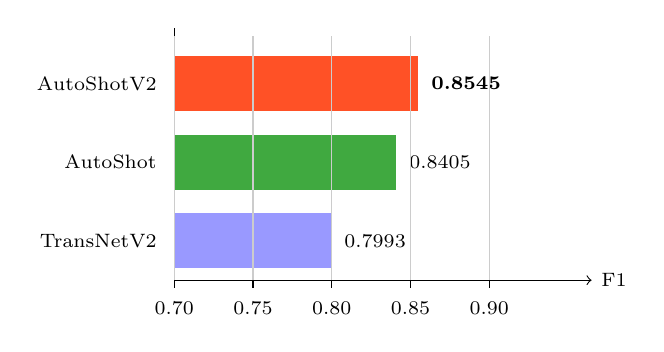
\begin{tikzpicture}[font=\small]
% Horizontal bar chart comparing F1 scores
% Scale: display_x = (value - 0.70) * 20
% [0.70, 0.95] → [0, 5] cm

% Bar heights (y centers) and half-height
\def\yA{2.4}  % AutoShotV2
\def\yB{1.4}  % AutoShot
\def\yC{0.4}  % TransNetV2
\def\hh{0.35}

% Bars
% TransNetV2 F1=0.7993 → (0.7993-0.7)*20=1.986
\fill[blue!50, opacity=0.8]        (0,\yC-\hh) rectangle (1.986,\yC+\hh);
% AutoShot F1=0.8405 → 2.810
\fill[green!55!black, opacity=0.75](0,\yB-\hh) rectangle (2.810,\yB+\hh);
% AutoShotV2 F1=0.8545 → 3.090
\fill[red!60!orange, opacity=0.85] (0,\yA-\hh) rectangle (3.090,\yA+\hh);

% Value labels
\node[anchor=west, font=\scriptsize]        at (2.036, \yC) {0.7993};
\node[anchor=west, font=\scriptsize]        at (2.860, \yB) {0.8405};
\node[anchor=west, font=\scriptsize\bfseries] at (3.140, \yA) {\textbf{0.8545}};

% Model name labels
\node[anchor=east, font=\scriptsize] at (-0.1, \yC) {TransNetV2};
\node[anchor=east, font=\scriptsize] at (-0.1, \yB) {AutoShot};
\node[anchor=east, font=\scriptsize] at (-0.1, \yA) {AutoShotV2};

% X-axis and ticks
\draw[->] (0,-0.1) -- (5.3,-0.1) node[right, font=\scriptsize] {F1};
\draw     (0,-0.1) -- (0,3.1);
\foreach \v/\x in {0.70/0, 0.75/1, 0.80/2, 0.85/3, 0.90/4} {
  \draw[gray!40, thin] (\x, -0.1) -- (\x, 3.0);
  \draw (\x,-0.1) -- (\x,-0.2);
  \node[below, font=\scriptsize] at (\x,-0.25) {\v};
}
\end{tikzpicture}
\caption[So sánh F1 trên tập SHOT]{So sánh F1 giữa các mô hình trên tập SHOT (200 video kiểm tra). AutoShotV2 đạt F1 = 0.8545, cải thiện $+1.4$ điểm phần trăm so với AutoShot gốc và $+5.5$ điểm phần trăm so với TransNetV2 mô hình cơ sở.}
\label{fig:f1_comparison}
\end{figure}
\FloatBarrier

\section{Hiệu chỉnh hậu xử lý theo dữ liệu bằng kiểm định chéo}
\label{sec:calibration}

Để củng cố nhận định về khoảng cách trên ClipShots một cách định lượng và tránh hiện tượng ``tinh chỉnh trên tập kiểm tra'', khóa luận bổ sung một thí nghiệm hiệu chỉnh hậu xử lý theo từng bộ dữ liệu bằng kiểm định chéo 5 phần (5-fold cross-validation). Các tham số hậu xử lý (nhiệt độ, $\sigma$ của Gaussian và ngưỡng quyết định) được chọn trên các phần hiệu chỉnh rồi đo trên phần giữ lại, nên F1 báo cáo không bị tinh chỉnh trên chính dữ liệu dùng để đo. Thí nghiệm chạy trên logits đã lưu, không huấn luyện lại.

\begin{table}[H]
\centering
\caption[F1 sau hiệu chỉnh hậu xử lý (kiểm định chéo)]{F1 triển khai sau hiệu chỉnh hậu xử lý theo từng bộ dữ liệu, đo bằng kiểm định chéo 5 phần (không tinh chỉnh trên tập kiểm tra). Số đậm là giá trị tốt nhất theo cột.}
\label{tab:calibration_cv}
\small
\begin{tabular}{lccc}
\toprule
\textbf{Mô hình} & \textbf{SHOT} & \textbf{BBC} & \textbf{ClipShots} \\
\midrule
\CalibrationCVRows
\bottomrule
\end{tabular}
\end{table}

\noindent
Ba kết luận có kiểm chứng:
\begin{itemize}
    \item \textbf{Hiệu chỉnh là một cải thiện rẻ.} Ngay cả baseline $A0$ cũng tăng đáng kể nhờ hiệu chỉnh theo từng bộ dữ liệu (ClipShots $0.7649 \rightarrow 0.7881$); tham số được chọn ổn định qua các phần ($\sigma=2$ gần như luôn được chọn), khớp với kết luận ablation rằng Gaussian smoothing là thành phần tác động lớn nhất.
    \item \textbf{Pha 2 giúp SHOT và BBC nhưng kém $A0$ trên ClipShots.} Sau hiệu chỉnh, Pha 2 vượt $A0$ trên SHOT ($0.854$ so với $0.844$) và BBC ($0.963$ so với $0.954$), nhưng vẫn thua trên ClipShots ($0.757$ so với $0.788$); hiệu chỉnh không bù được khoảng cách này. Đây là bằng chứng định lượng cho nhận định khả năng tổng quát hóa sang ClipShots chưa được giải quyết bằng fine-tune hiện tại.
    \item \textbf{Khoảng chênh lạc quan nhỏ.} Mức trần khi tinh chỉnh trực tiếp trên tập kiểm tra rất sát với số kiểm định chéo (ví dụ ClipShots $A0$: $0.7896$ so với $0.7881$), cho thấy quá trình hiệu chỉnh ổn định và không bị overfit.
\end{itemize}

\section{Phân tích lỗi và khả năng tổng quát hóa}

\subsection{Breakdown theo bộ dữ liệu}
Kết quả cho thấy SHOT là tập dữ liệu mà AutoShotV2 đạt F1 cao nhất, trong khi ClipShots suy giảm đáng kể. Xu hướng này nhất quán với đặc điểm dữ liệu đã mô tả ở phần đầu chương: SHOT có nhịp cảnh nhanh và phân phối gần với dữ liệu dùng để tinh chỉnh tầng phân loại, còn ClipShots có miền nội dung đa dạng hơn, nhiều hiệu ứng chuyển cảnh ``hoang dã'' và điều kiện ghi hình không đồng nhất.

Với BBC, mô hình giữ mức F1 cao nhưng không còn vượt trội khi so với cấu hình gốc. Điều này gợi ý rằng các kỹ thuật hậu xử lý đang ưu tiên phân phối của video ngắn nhiều hơn là phân phối video tài liệu dài.

\subsection{Giải thích suy giảm trên ClipShots}

Bảng~\ref{tab:clipshots_breakdown} phân tách F1 của AutoShotV2 trên ClipShots theo loại chuyển cảnh, làm rõ nguyên nhân suy giảm. Bảng này dùng ngưỡng 0.10 để phân tích lỗi theo loại chuyển cảnh, khác với ngưỡng quét (sweep) 0.15 dùng cho kết quả tổng hợp ở Bảng~\ref{tab:autoshotv2_prf}.

\begin{table}[H]
\centering
\caption[Breakdown theo loại chuyển cảnh trên ClipShots]{Breakdown Precision/Recall/F1 theo loại chuyển cảnh trên ClipShots test (500 video, ngưỡng = 0.10).}
\label{tab:clipshots_breakdown}
\small
\begin{tabular}{lccc}
\toprule
\textbf{Loại chuyển cảnh} & \textbf{Precision} & \textbf{Recall} & \textbf{F1} \\
\midrule
Cut (chuyển cảnh đột ngột) & 0.5826 & 0.8860 & 0.7030 \\
Gradual (chuyển cảnh dần) & 0.6456 & 0.0442 & 0.0828 \\
\textbf{Tổng}              & \textbf{0.7477} & \textbf{0.7897} & \textbf{0.7681} \\
\bottomrule
\end{tabular}
\end{table}

\noindent
Độ bao phủ của loại \textit{gradual} (độ bao phủ chuyển cảnh dần) chỉ đạt $4.42\%$ -- mô hình gần như không phát hiện được các chuyển cảnh dần trên ClipShots. Đây là nguyên nhân chính kéo F1 tổng thể xuống thấp hơn so với SHOT.

Mức giảm $3.1$ điểm phần trăm so với AutoShot theo báo cáo gốc trên ClipShots, kết hợp với độ bao phủ ranh giới dần (độ bao phủ chuyển cảnh dần) cực thấp ở Bảng~\ref{tab:clipshots_breakdown}, gợi mở ba giả thuyết kỹ thuật cần kiểm chứng thêm:
\begin{enumerate}
    \item \textbf{Many-hot $\pm 1$ frame có thể chưa phù hợp với chuyển cảnh đột ngột sắc của ClipShots:} Khi phần lớn ranh giới ClipShots là chuyển cảnh đột ngột rất sắc, việc mở rộng nhãn dương ra $\pm 1$ frame có thể làm ``dày'' vùng dương hơn mức cần thiết và làm mềm độ sắc quyết định biên --- một hiệu ứng mà many-hot không gây ra trên SHOT vì SHOT có tỉ lệ chuyển cảnh dần (chuyển cảnh dần) cao hơn.
    \item \textbf{Hiệu chỉnh nhiệt độ (Temperature scaling) tối ưu trên validation SHOT có thể không tổng quát hóa sang miền khác:} $T^* = 0.3878$ được tìm trên tập xác thực của SHOT; khi phân phối logit của mô hình trên ClipShots khác đi, cùng một hệ số có thể làm phân phối xác suất bị lệch và đẩy ngưỡng tối ưu sang vùng không ổn định.
    \item \textbf{Cấu hình Focal Loss có thể thiên về phân phối nhãn của SHOT:} Bộ $\gamma=1.0,\alpha=0.5$ được chọn qua tìm kiếm lưới trên SHOT; do tỉ lệ chuyển cảnh và độ khó mẫu trên ClipShots khác, cấu hình này chưa chắc là tối ưu cho miền đa dạng hơn.
\end{enumerate}

Cả ba giả thuyết trên đều cần thí nghiệm đối chứng tách biệt từng yếu tố (ví dụ: chạy lại AutoShotV2 không many-hot, hoặc dùng $T^*$ tính lại trên tập xác thực của ClipShots) để loại trừ các nhân tố khác --- đây là hạn chế thực nghiệm của khóa luận, được nêu lại ngay ở mục tiếp theo.

\subsection{Giới hạn của phân tích hiện tại}
Các giả thuyết trên được xây dựng từ số liệu F1/Precision/Recall hiện có, chưa đi kèm thí nghiệm đối chứng tách biệt từng yếu tố. Do không chạy lại toàn bộ ma trận thử nghiệm phân rã trên mọi tập dữ liệu trong phạm vi khóa luận, kết luận ở đây nên được xem là định hướng phân tích có cơ sở, và cần kiểm chứng thêm trong công việc tương lai.

\section{Trả lời câu hỏi nghiên cứu}
\label{sec:ch5_rq_results}

\subsection{Trả lời các câu hỏi nghiên cứu}
\label{sec:rq_answers}
Các kết quả thực nghiệm trong chương này cho phép trả lời trực tiếp ba câu hỏi nghiên cứu đã được đặt ra ở Mục~\ref{sec:research_questions}.

\begin{itemize}
    \item \textbf{RQ1:} \textit{Có} --- AutoShot vượt TransNetV2 $+4.12$ điểm phần trăm F1 trên SHOT (Bảng~\ref{tab:autoshotv2_results}), xác nhận lợi ích của NAS cho video ngắn.
    \item \textbf{RQ2:} \textit{Có} --- AutoShotV2 đạt F1 = \ASVTwoShotFOne{} trên SHOT ($+\ASVTwoVsAutoShotShotPP$ so với AutoShot, $+\ASVTwoVsTransNetShotPP$ so với TransNetV2) chỉ bằng cải tiến tầng phân loại, không thay đổi mạng xương sống.
    \item \textbf{RQ3:} \textit{Một phần} --- vượt mô hình cơ sở trên BBC (F1 = \ASVTwoBBCFOne) nhưng suy giảm trên ClipShots (F1 = \ASVTwoClipFOne), chủ yếu do độ bao phủ ranh giới dần (độ bao phủ chuyển cảnh dần) chỉ đạt $4.4\%$ (Bảng~\ref{tab:clipshots_breakdown}).
\end{itemize}

\subsection{Phát hiện bổ sung ngoài phạm vi RQ}
Bên cạnh ba câu trả lời cho RQ ở trên, thí nghiệm còn cho thấy một số quan sát đáng chú ý ở tầng phương pháp luận và triển khai:

\begin{itemize}
    \item \textbf{SHOT là phép thử khó nhưng sát thực tế video ngắn.} So với BBC, RAI và ClipShots, SHOT có shot ngắn hơn (TB $2.59$~s) và nhiều hiệu ứng chuyển cảnh phức tạp hơn; do đó là chuẩn đánh giá phù hợp hơn cho môi trường TikTok/Reels/Shorts so với các chuẩn đánh giá video dài truyền thống.
    \item \textbf{NAS đắt nhưng có thể tái sử dụng.} Chi phí tìm kiếm kiến trúc và huấn luyện lại với KD/Weight Grafting đáng kể, nhưng AutoShotV2 cho thấy mạng xương sống đã tìm được có thể dùng lại nhiều lần cho các cải tiến ở tầng phân loại với chi phí phụ trội rất nhỏ --- một mô hình triển khai khả thi cho phòng lab có tài nguyên hạn chế.
    \item \textbf{Ngưỡng suy luận là tham số ứng dụng, không phải tham số mô hình.} Ngưỡng tối ưu theo F1 cho cân bằng Precision--Recall tốt nhất; ngưỡng cao hơn ưu tiên Precision khi đánh đổi Recall. Lựa chọn ngưỡng nên căn cứ vào yêu cầu nghiệp vụ cuối (số lượng dương tính giả chấp nhận được trong workflow biên tập), không nhất thiết phải là một con số tuyệt đối.
\end{itemize}
\section{Tổng kết chương}
Chương này đã trình bày kết quả đánh giá AutoShotV2 trên SHOT, BBC và ClipShots; phân tích chi tiết Precision/Recall/F1; kiểm tra đóng góp của từng thành phần thông qua phân rã; và thảo luận các lỗi còn tồn tại khi chuyển miền dữ liệu. Các kết quả cho thấy cải tiến ở tầng phân loại có thể hỗ trợ tốt cho mạng xương sống AutoShot trên miền video ngắn, nhưng khả năng tổng quát hóa sang dữ liệu đa dạng hơn vẫn là hạn chế cần tiếp tục nghiên cứu. Chương~\ref{chuong6} sẽ tổng kết toàn bộ khóa luận, nêu hạn chế và hướng phát triển tương lai.




